%----------------------------------------------------------------------------------------------------------------------
\begin{frame}{Context}
\begin{itemize}[noitemsep,label=\textbullet,topsep=2pt,parsep=2pt,partopsep=2pt]
\item Product Development: A quicker validation is crucial; fierce competition; faster obsolescence.
\item Trend: Digital instead of Physical prototyping
\item Meaning: Modeling by CAD and analysis by CAE
\item How: More robust, quicker the CAD-CAE transition, faster is the product development, and design iterations
\item Solution: Use of `Model Simplification', De-featuring and Dimension Reduction.
\item  In the age of scalable and near-infinite computing power, for more design iterations quickly. 
\end{itemize}

%Notes: 

\end{frame}

%----------------------------------------------------------------------------------------------------------------------
\begin{frame}{Specific solution}
\begin{itemize}[noitemsep,label=\textbullet,topsep=2pt,parsep=2pt,partopsep=2pt]
\item Domain:`thin-walled models' i.e. Sheet Metal, Plastics etc
\item Expensive 3D elements, 2D elements on midsurface
\item Fairly accurate results in lesser computations/time.

\vspace{1cm}

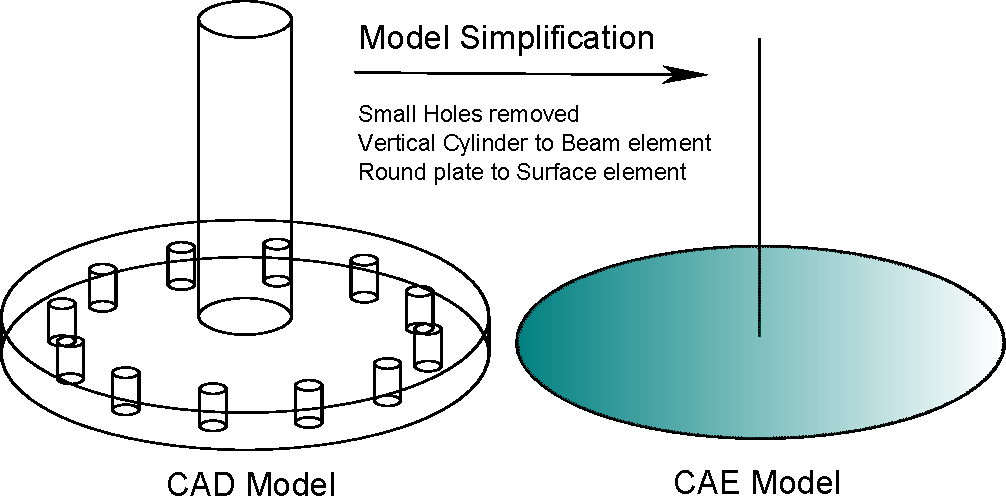
\includegraphics[width=0.8\linewidth]{../Common/images/ModelSimplification.pdf}
\end{itemize}

%Notes: 

\end{frame}


%----------------------------------------------------------------------------------------------------------------------
\begin{frame}{What is Midsurface?}
\begin{itemize}[noitemsep,label=\textbullet,topsep=2pt,parsep=2pt,partopsep=2pt]
\item A surface lying midway of a thin-walled solid, mimicking its shape.
\item Surface representation/idealization/abstraction along with thickness data
\item Not expected to work for thick models

\vspace{1cm}

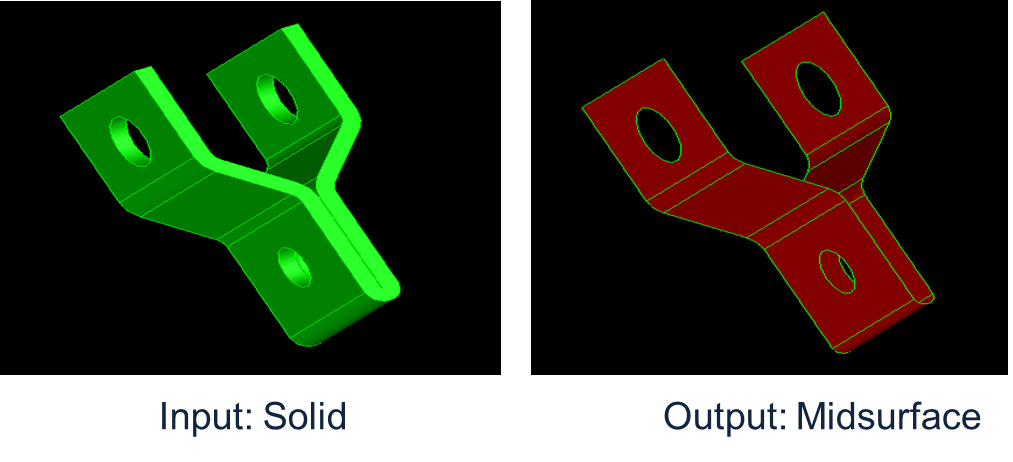
\includegraphics[width=0.85\linewidth]{../Common/images/SolidToMidsurface.png}
\end{itemize}

%Notes: 

\end{frame}


%----------------------------------------------------------------------------------------------------------------------
\begin{frame}{What is the problem?}
\begin{itemize}[noitemsep,label=\textbullet,topsep=2pt,parsep=2pt,partopsep=2pt]
\item Gaps, Missing patches,  Not lying midway

\vspace{0.25cm}

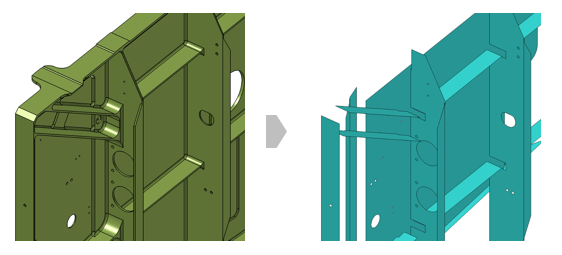
\includegraphics[width=0.85\linewidth]{../Common/images/MidsurfaceErrorsMscApex}

\item  Automated and  robust technique  is a crucial need
\end{itemize}

%Notes: 

\end{frame}

%----------------------------------------------------------------------------------------------------------------------
\begin{frame}{Research Potential}
\begin{itemize}[noitemsep,label=\textbullet,topsep=2pt,parsep=2pt,partopsep=2pt]
\item Widely used but not robust
\item Uses final Brep (due to legacy) and not features
\item Research is still going on...(July 2015)

\vspace{1cm}
%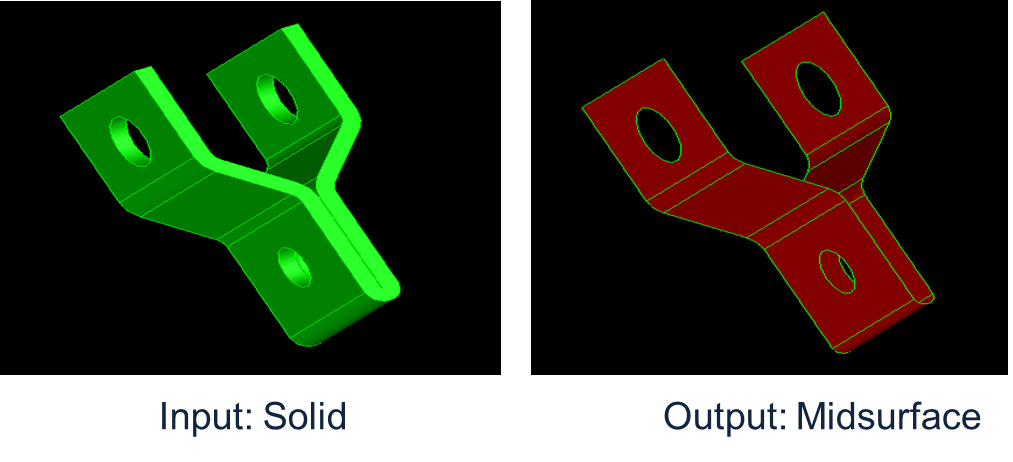
\includegraphics[scale=0.5]{../Common/images/SolidToMidsurface.png}
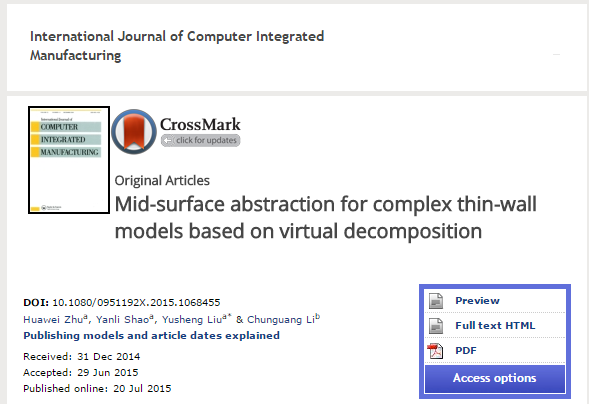
\includegraphics[width=0.65\linewidth]{../Common/images/latestmidsurf1}
\end{itemize}

%Notes: 

\end{frame}


%----------------------------------------------------------------------------------------------------------------------
\begin{frame}{Where do you find Thin Wall models?}
\vspace{1cm}

%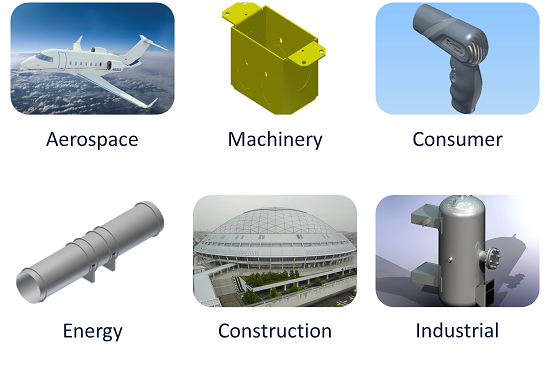
\includegraphics[scale=0.5]{../Common/images/ThinWallApplications.png}
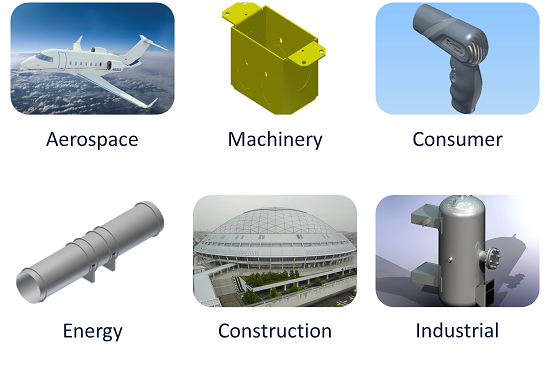
\includegraphics[width=0.85\linewidth]{../Common/images/ThinWallApplications.png}

%Notes: 

\end{frame}


%----------------------------------------------------------------------------------------------------------------------
\begin{frame}{What is considered as {\bf Thin}?}
It is defined as a part or body with large effective span to  thickness ratio ($L/T$)

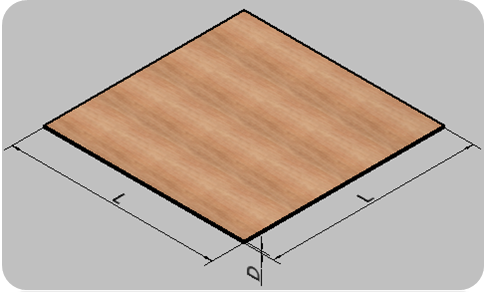
\includegraphics[scale=0.25]{../Common/images/WhatIsThin.png}

For 'Thin', Solid and Shell elements give comparable results
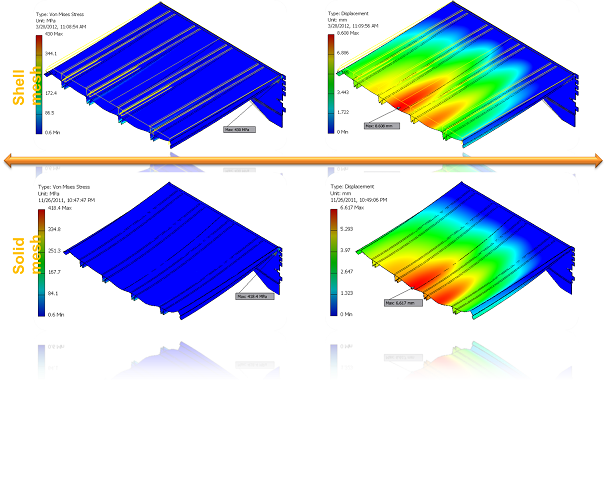
\includegraphics[scale=0.25]{../Common/images/ShellSolid.png}

%Notes: 

\end{frame}

%
%----------------------------------------------------------------------------------------------------------------------
%\begin{frame}{What is considered as {\bf Thin}?}
%It is defined as a part or body with large effective span to  thickness ratio ($L/T$)
%
%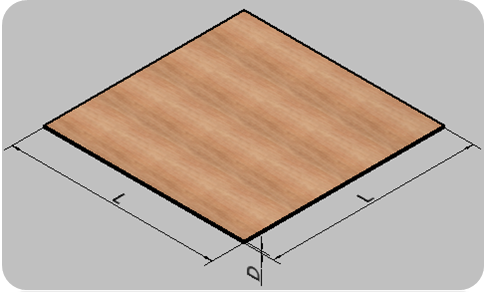
\includegraphics[scale=0.25]{../Common/images/WhatIsThin.png}
%
%For 'Thin', Solid and Shell elements give comparable results
%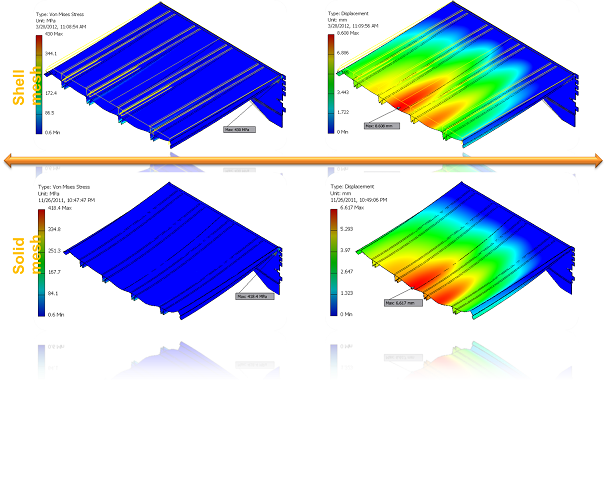
\includegraphics[scale=0.3]{../Common/images/ShellSolid.png}
%
%%Notes: 
%
%\end{frame}

%----------------------------------------------------------------------------------------------------------------------
%
\begin{frame}{Classification of Thin-ness}
Thickness threshold is based on the Length to Thickness ratio  $L/T$ 

\begin{itemize}[noitemsep,label=\textbullet,topsep=2pt,parsep=2pt,partopsep=2pt]
\item Length = Overall length of the input solid body
\item Thickness = Thickness of the input solid body
\end{itemize}
%\begin{table}[!h]
\begin{tabular}[h]{@{}l l l  @{}}
\toprule

{\bf $L/T$  ratio } & {\bf Interpretation } & {\bf Element}\\
\midrule
$L/T < 100$ & Body is thick & Solid \\
$L/T \geq 100$ \& $L/T \leq 250$ & Body may be thin & Shell or Solid \\
$L/T > 250$ \& $L/T \leq 750$ & Body is thin & Shell \\
$L/T > 750$ & Body is too thin & Certainly Shell \\
\bottomrule
\end{tabular}
%\end{table}


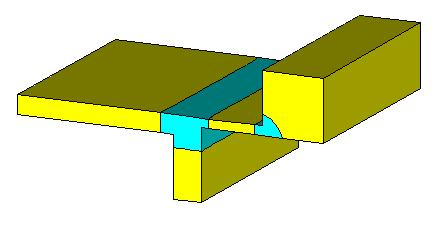
\includegraphics[scale=0.4]{../Common/images/PriceThin.jpg}

\end{frame}


%----------------------------------------------------------------------------------------------------------------------

\begin{frame}{But why not just one side of it?}
\begin{itemize}[noitemsep,label=\textbullet,topsep=2pt,parsep=2pt,partopsep=2pt]
\item Midsurface is needed to follow shape of the base part as well as carry thickness information. It should not be biased towards one of the sides.
\item Figure shows two configurations for 'L' shape. Irrespective of the way they have been joined, CAE would like to have surface that would follow the base part shape and look like proper 'L'. If any of the sides are taken, results are skewed.

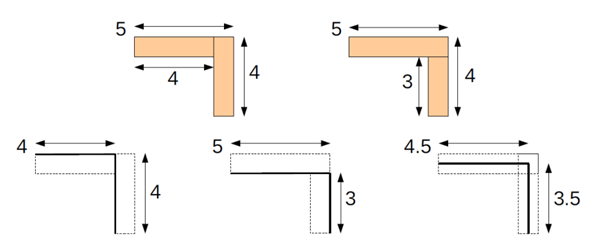
\includegraphics[scale=0.5]{../Common/images/OneSide.png}

\end{itemize}

%Notes: 

\end{frame}

%----------------------------------------------------------------------------------------------------------------------

\begin{frame}{Effect of Thickness on Side-ness}
\begin{itemize}[noitemsep,label=\textbullet,topsep=2pt,parsep=2pt,partopsep=2pt]
\item Shell elements are meshed on surfaces (compared to solids in volumes)
\item COSMOS [SolidWorks] understands the shell placement to ALWAYS be at the Midsurface of the part
\begin{itemize}[noitemsep,label=\textbullet,topsep=2pt,parsep=2pt,partopsep=2pt]
\item For convenience, it may be easier to choose an inside or outside part surface
\item The higher the part aspect ratio, the less it matters
\end{itemize}

\vspace{0.5cm}

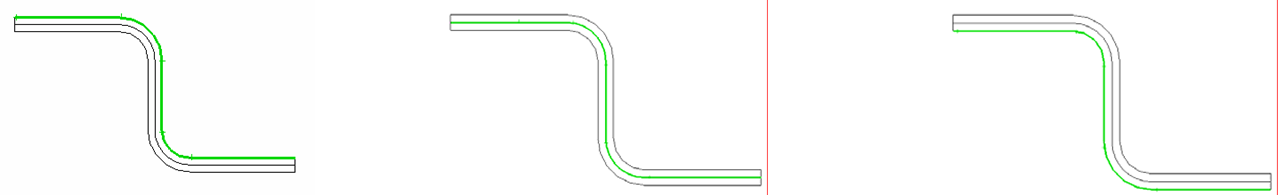
\includegraphics[scale=0.45]{../Common/images/EffectOfThickness.png}

\end{itemize}

\end{frame}



%----------------------------------------------------------------------------------------------------------------------

\begin{frame}{Methods for Midsurface computation}
\begin{itemize}[noitemsep,label=\textbullet,topsep=2pt,parsep=2pt,partopsep=2pt]
\item Midsurface Abstraction (MA) Approach and Medial Axis Transform (MAT) Approach are based on Extraction, meaning the algorithm is applied on the ready-final model to extract Midsurface. 

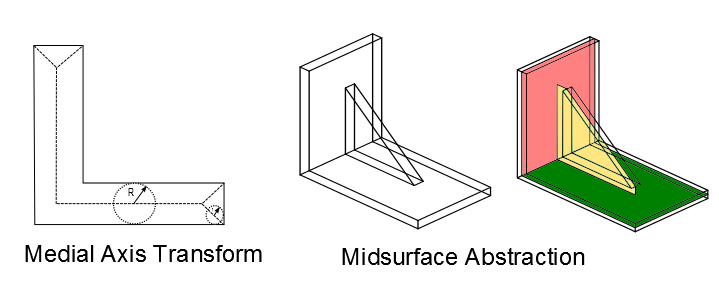
\includegraphics[scale=0.25]{../Common/images/MAT_Midsurf.png}

\item Many a times due to complexity in recognizing forms, their interactions, same design-intent used while modeling part can not be applied to Midsurface and thus Midsurface of part does not follow its form and connectivity

\item Idea is to leverage the design intent in the form of feature history tree, to build the Midsurface as the way model gets built, step by step.
\end{itemize}

%Notes: 

\end{frame}

